\documentclass{article}

\usepackage{graphicx}
\usepackage{tikz}
\usepackage{tikzsymbols}
\usetikzlibrary{calc,patterns,shapes.geometric}
\pagestyle{empty}
\usepackage[margin=0pt]{geometry}
\geometry{papersize={14in,12in}}

\def\centerarc[#1](#2)(#3:#4:#5){\draw[#1] ($(#2)+({#5*cos(#3)},{#5*sin(#3)})$) arc (#3:#4:#5);}

\begin{document}
	\begin{figure}
		\centering
		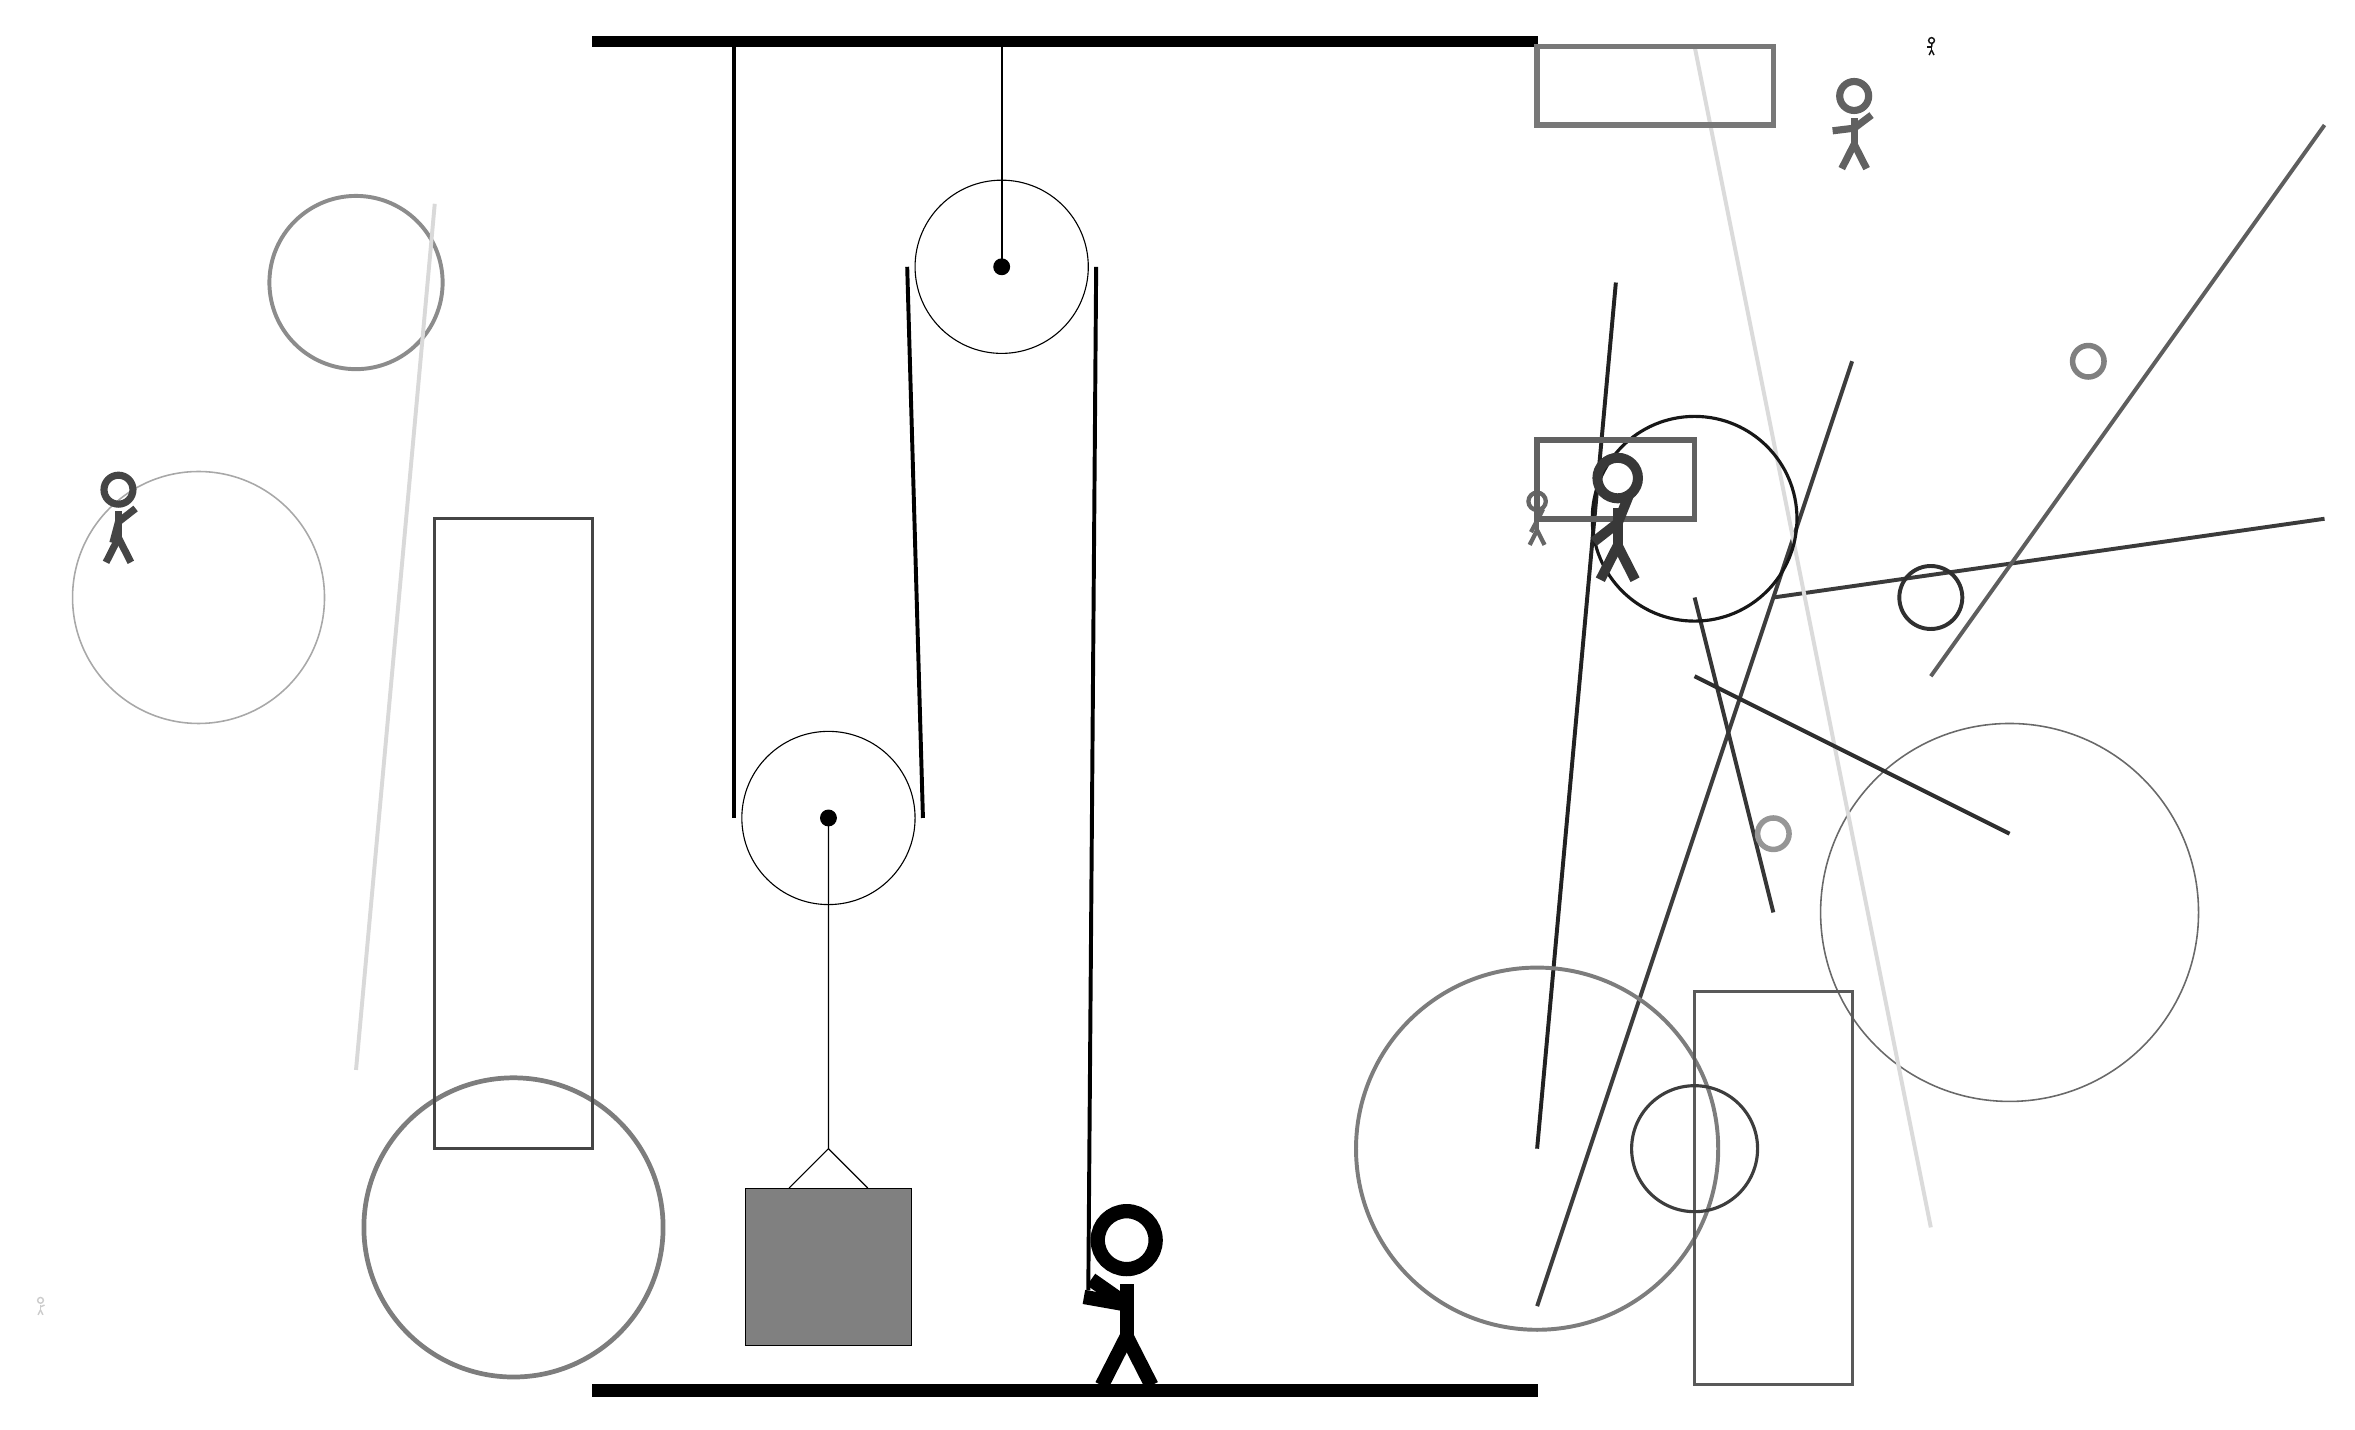
\begin{tikzpicture}
			%%%%% START %%%%%
			
			\draw[fill=black] (-2, 14) rectangle (10, 14.125);
			
			\draw (3.2, 11.2) circle (1.1);
			\draw[fill=black] (3.2, 11.2) circle (0.1);
			\draw[thick] (3.2, 11.2) -- (3.2, 14);
			
			\draw (1, 4.2) circle (1.1);
			\draw[fill=black] (1, 4.2) circle (0.1);
			
			\draw (1, 4.2) -- (1, 0) -- (0.5, -0.5);
			\draw (1, 0) -- (1.5, -0.5);
			\draw[fill=black!50] (-0.05, -0.5) rectangle (2.05, -2.5);
			
			\draw[line width=0.5mm] (-0.2, 14) -- (-0.2, 4.2);
			\centerarc[line width=0.5mm](1, 4.2)(180:360:1.2000000000000002);
			\draw[line width=0.5mm](2.2, 4.2) -- (2.0, 11.2);
			\centerarc[line width=0.5mm](3.2, 11.2)(0:180:1.2000000000000002);
			\draw[line width=0.5mm](4.4, 11.2) -- (4.3, -1.8);
			
			\node[line width=0.7mm, color=black!60] at (10, 8) {\Strichmaxerl[3][62][63]};
			
			\draw [line width=0.5mm, color=black!45](-5, 11) circle (1.1);
			\draw [line width=0.2mm, color=black!59](16, 3) circle (2.4);
			\draw[line width=0.5mm, color=black!87](11, 11) -- (10, 0);
			\draw [line width=0.2mm, color=black!34](-7, 7) circle (1.6);
			\draw[line width=0.5mm, color=black!76](10, -2) -- (14, 10);
			\draw [line width=0.5mm, color=black!51](10, 0) circle (2.3);
			\draw[line width=0.5mm, color=black!15](-4, 12) -- (-5, 1);
			\draw[line width=0.5mm, color=black!77](13, 7) -- (20, 8);
			\node[line width=0.7mm, color=black!62] at (14, 13) {\Strichmaxerl[5][7][37]};
			
			\draw[line width=0.5mm, color=black!14](15, -1) -- (12, 14);
			\draw[line width=0.7mm, color=black!53] (10, 14) rectangle (13, 13);
			\draw[line width=0.5mm, color=black!79](12, 7) -- (13, 3);
			
			\draw[line width=0.4mm, color=black!65] (12, 2) rectangle (14, -3);
			\node[line width=0.5mm, color=black!73] at (-8, 8) {\Strichmaxerl[5][75][38]};
			\draw [line width=0.4mm, color=black!91](12, 8) circle (1.3);
			\draw [line width=0.6mm, color=black!51](-3, -1) circle (1.9);
			\draw[line width=0.7mm, color=black!62] (10, 8) rectangle (12, 9);
			\draw [line width=0.4mm, color=black!64](-5, 5) circle (0.0);
			
			\draw [line width=0.7mm, color=black!50](17, 10) circle (0.2);
			\draw [line width=0.7mm, color=black!41](13, 4) circle (0.2);
			
			\draw[line width=0.5mm, color=black!63](15, 6) -- (20, 13);
			\node[line width=0.6mm, color=black!93] at (15, 14) {\Strichmaxerl[1][0][81]};
			\node[line width=0.2mm, color=black!78] at (11, 8) {\Strichmaxerl[7][38][68]};
			\node[line width=0.2mm, color=black!20] at (-9, -2) {\Strichmaxerl[1][90][23]};
			\draw [line width=0.4mm, color=black!76](12, 0) circle (0.8);
			\draw[line width=0.5mm, color=black!82](12, 6) -- (16, 4);
			\draw[line width=0.3mm, color=black!47] (-2, 1) rectangle (-2, 0);
			
			\draw [line width=0.5mm, color=black!81](15, 7) circle (0.4);
			\draw[line width=0.4mm, color=black!73] (-2, 0) rectangle (-4, 8);
			
			\node at (4.7, -1.9) {\Strichmaxerl[10][-35][170]};
			
			\draw[fill=black] (-2, -3) rectangle (10, -3.15);
			
			%%%%% END %%%%%
		\end{tikzpicture}
	\end{figure}	
\end{document}